\chapter{Conclusion} \label{chapter7}
\minitoc
\eject

The web brought a new economic model allowing a tremendous number of business opportunities.
To seize these opportunities, a team needs to develop a web application, and grow a business around it.
The economical incentives around the technical development changes completely during the growth of this business.
In the beginning, the development needs to be productive, to quickly release a product and iterate with the user feedbacks.
When the project matures, the execution needs to be efficient, to cope with the load of a large user base while limiting the hardware costs.

These two development concerns are incompatible.
No platform can provide both performance efficiency, and development productivity at the same time.
The platforms at the state of the art propose only a fixed compromise between the two.
This thesis presented a platform allowing an evolutive compromise to fit the economical incentives.

\subsection{Real test case} \label{chapter5:flx:evaluation}

The compiler is tested on a real application, gifsockets-server\ftnt{https://github.com/twolfson/gifsockets-server}.
This test proves the possibility for an application to be compiled into a network of independent parts.
It shows the current limitations of this isolation and the modifications needed on the application to circumvent them.

\begin{code}[js, caption={Simplified version of gifsockets-server},label={lst:gifsocket}]
var express = require('express'),
    app = express(),
    routes = require('gifsockets-middleware'), //@\label{lst:gifsocket:gif-mw}@
    getRawBody = require('raw-body');

function bodyParser(limit) { //@\label{lst:gifsocket:bodyParser}@
  return function saveBody(req, res, next) { //@\label{lst:gifsocket:saveBody}@
    getRawBody(req, { //@\label{lst:gifsocket:getRawBody}@
      expected: req.headers['content-length'],
      limit: limit
    }, function (err, buffer) { //@\label{lst:gifsocket:callback}@
      req.body = buffer;
      next(); //@\label{lst:gifsocket:next}@
    });
  };
}

app.post('/image/text', bodyParser(1 * 1024 * 1024), routes.writeTextToImages); //@\label{lst:gifsocket:app.post}@
app.listen(8000);
\end{code}

This application, simplified in listing \ref{lst:gifsocket}, is a real-time chat using gif-based communication channels.
It was selected from the evaluation set of the Due compiler because it is simple enough to illustrate this evaluation.
% \cite{Brodu2015}
%  from the \texttt{npm} registry because it depends on \texttt{express}, it is tested, working, and simple enough to illustrate this evaluation.
The server transforms the received text into a gif frame, and pushes it back to a never-ending gif to be displayed on the client.

On line \ref{lst:gifsocket:app.post}, the application registers two functions to process the requests received on the url \texttt{/image/text}.
The closure \texttt{saveBody}, line \ref{lst:gifsocket:saveBody}, returned by \texttt{bodyParser}, line \ref{lst:gifsocket:bodyParser}, and the method \texttt{routes.write\-Text\-To\-Images} from the external module \texttt{gifsockets-\-middleware}, line \ref{lst:gifsocket:gif-mw}.
The closure \texttt{saveBody} calls the asynchronous function \texttt{getRawBody} to get the request body.
Its callback handles the errors, and calls \texttt{next} to continue processing the request with the next function, \texttt{routes.write\-Text\-To\-Images}.

\subsubsection{Compilation} \label{chapter5:flx:evaluation:compilation}

% We compile this application with the compiler
The compilation result is in listing \ref{lst:flx-gifsocket}.
The function call \texttt{app.post}, line \ref{lst:gifsocket:app.post}, is a rupture point.
However, its callbacks, \texttt{bodyParser} and \texttt{routes.write\-Text\-To\-Images} are not declared \textit{in situ}.
They are evaluated as functions only at runtime.
As precised previously, the compiler discards these callbacks to avoid altering the semantic. % by moving or modifying their definition.
% For this reason, the compiler ignores this rupture point, to avoid interfering with the evaluation.

\begin{code}[flx, caption={Compilation result of gifsockets-server},label={lst:flx-gifsocket}]
flx main & express {req}
>> anonymous_1000 [req, next]
  var express = require('express'),
      app = express(),
      routes = require('gifsockets-middleware'), //@\label{lst:flx-gifsocket:gif-mw}@
      getRawBody = require('raw-body');

  function bodyParser(limit) { //@\label{lst:flx-gifsocket:bodyParser}@
    return function saveBody(req, res, next) { //@\label{lst:flx-gifsocket:saveBody}@
      getRawBody(req, { //@\label{lst:flx-gifsocket:getRawBody}@
        expected: req.headers['content-length'], //@\label{lst:flx-gifsocket:req.headers}@
        limit: limit
      }, >> anonymous_1000 [req, next]);
    };
  }

  app.post('/image/text', bodyParser(1 * 1024 * 1024), routes.writeTextToImages); //@\label{lst:flx-gifsocket:app.post}@
  app.listen(8000);

flx anonymous_1000
-> null
  function (err, buffer) { //@\label{lst:flx-gifsocket:callback}@
    req.body = buffer; //@\label{lst:flx-gifsocket:buffer}@
    next(); //@\label{lst:flx-gifsocket:next}@
  }
\end{code}

The compiler detects a rupture point : the function \texttt{get\-Raw\-Body} and its anonymous callback, line \ref{lst:gifsocket:callback}.
It encapsulates this callback in a fluxion named \texttt{anony\-mous\_\-1000}.
The callback is replaced with a stream placeholder to send the message stream to this downstream fluxion.
The variables \texttt{req} and \texttt{next} are appended to this message stream, to propagate their value from the \texttt{main} fluxion to the \texttt{anony\-mous\_\-1000} fluxion.

When \texttt{anony\-mous\_\-1000} is not isolated from the \texttt{main} fluxion, as if they belong to the same group, the compilation result works as expected.
The variables used in the fluxion, \texttt{req} and \texttt{next}, are still shared between the two fluxions.
In this situation fluxions are quite similar to Dues regarding memory shareing.
Our goal is to isolate the two fluxions, to be able to safely parallelize their executions.

\subsubsection{Isolation} \label{chapter5:flx:evaluation:isolation}

In listing \ref{lst:flx-gifsocket}, the fluxion \texttt{anony\-mous\_\-1000} modifies the object \texttt{req}, line \ref{lst:flx-gifsocket:buffer}, to store the text of the received request, and it calls \texttt{next} to continue the execution, line \ref{lst:flx-gifsocket:next}.
\texttt{req} is an alias to a memory location used in multiple palces in code.
Therefore, these operations produce side-effects that should propagate in the whole application, but the isolation prevents this propagation.
Isolating the fluxion \texttt{anony\-mous\_\-1000} produces runtime exceptions.
The next paragraph details how this situation is handled to allow the application to be parallelized.

\paragraph{Variable \texttt{req}}

The variable \texttt{req} is read in fluxion \texttt{main}, lines \ref{lst:flx-gifsocket:getRawBody} and \ref{lst:flx-gifsocket:req.headers}.
Then its property \texttt{body} is associated to \texttt{buffer} in fluxion \texttt{anony\-mous\_\-1000}, line \ref{lst:flx-gifsocket:buffer}.
The compiler is unable to identify the aliases of this variable. % further usages.
However, the side effect resulting from this association impacts a variable in the scope of the next callback, \texttt{routes.write\-Text\-To\-Images}.
In this test case, the application is modified manually to explicitly propagate this side-effect to the next callback through the function \texttt{next}.
The modifications of this function are explained further in the next paragraph.

\paragraph{Closure \texttt{next}}

The function \texttt{next} is a closure provided by the \texttt{express} \texttt{Router} to continue the execution with the next function to handle the client request.
Because it indirectly relies on the variable \texttt{req}, it is impossible to isolate its execution with the \texttt{anony\-mous\_\-1000} fluxion.
Instead, we modify \texttt{express}, so as to be compatible with the fluxional execution model.
We explain the modifications below.

\begin{code}[flx, caption={Simplified modification on the compiled result},label={lst:mflx-gifsocket}]
flx anonymous_1000
-> express_dispatcher
  function (err, buffer) { //@\label{lst:mflx-gifsocket:callback}@
    req.body = buffer; //@\label{lst:mflx-gifsocket:buffer}@
    next_placeholder(req, -> express_dispatcher); //@\label{lst:mflx-gifsocket:next-placeholder}@
  }

flx express_dispatcher & express {req} //@\label{lst:mflx-gifsocket:express-dispatcher}@
-> null
  function (modified_req) {
    merge(req, modified_req);
    next(); //@\label{lst:mflx-gifsocket:next}@
  }
\end{code}

In listing \ref{lst:gifsocket}, the function \texttt{next} is a continuation allowing the anonymous callback, line \ref{lst:gifsocket:callback}, to call the next function to handle the request.
To isolate the anonymous callback into \texttt{anonymous\_\-1000}, \texttt{next} is replaced by a rupture point.
This replacement is illustrated in listing \ref{lst:mflx-gifsocket}.
The \texttt{express} \texttt{Router} registers a fluxion named \texttt{express\_\-dispatcher}, line \ref{lst:mflx-gifsocket:express-dispatcher}, to continue the execution after the fluxion \texttt{anony\-mous\_\-1000}.
This fluxion is in the same group \texttt{express} as the \texttt{main} fluxion, hence it has access to the original variable \texttt{req}, and to the original function \texttt{next}.
The call to the original \texttt{next} function is replaced by a placeholder to push the stream to the fluxion \texttt{express\_\-dispatcher}, line \ref{lst:mflx-gifsocket:next-placeholder}.
The fluxion \texttt{express\_\-dispatcher} receives the stream from the upstream fluxion \texttt{anony\-mous\_\-1000}, merges back the modification in the variable \texttt{req} to propagate the side effects, and finally calls the original function \texttt{next} to continue the execution, line \ref{lst:mflx-gifsocket:next}.

After the modifications detailed above, the server works as expected.
The isolated fluxion correctly receives, and returns its serialized messages.
The client successfully receives a gif frame containing the text.



\subsection{Limitations}

The static analysis used for this compiler presents some limitations.
It is unable to analyze code with dynamic behaviors.
Higher-order programming leads to more productivity partly beacuse it rely on such dynamic behavior to extend expressivity.
Precisely, it allows more levels of indirections.

\subsubsection{Levels of Indirections}

The indirection is an abstraction between the value, and its manipulation.
In listing \ref{lst:indirection}, the variables \texttt{a} and \texttt{b} point both to the same memory object.
The function \texttt{fn} introduces a level of indirection between the real object \texttt{a} and its manipulation handle, \texttt{b};
% Actually, the variable \texttt{a} already introduces a level of indirection between the real object and the handle \texttt{a}.

\begin{code}[js,
  caption={One level of Indirection},
  label={lst:indirection}]
var a = {
      // an object;
    };

fn(b) {
  // modify b;
}

fn(a);
\end{code}

\subsubsection{Uncertainties}

The indirection is trivial to resolve in listing \ref{lst:indirection}.
It only needs to have access to the definition of \texttt{a} and of \texttt{fn}.
%A very simple static analysis could resolve it.
However, in listing \ref{lst:indirections}, the array \texttt{handlers} introduces a new level of indirection.
The static analysis now needs to have access to the definition of \texttt{i} and of the \texttt{handlers}.
If this definition is provided by an external input, it is not available statically, hence, it adds an uncertainty during the analysis. 

\begin{code}[js,
  caption={Two levels of indirection},
  label={lst:indirections}]
var a = {
      // an object;
    },
    handlers = [
      // definition of fn handlers;
    ],
    i = ?;

handlers[i](a);
handlers[i+1](a);
\end{code}

These examples are extremely simplified.
A real application contains enough indirections for the static analysis to be overwhelmed by uncertainties, and to be unable to resolve the variables.
If a variable is left unresolved, it is impossible to assure its scope and its aliases.
Therefore, the compiler is unable to isolate it into a fluxion, or to distribute its modification by messages.

Moreover, it leads the compiler to ignore the rupture points not defined \textit{in situ}, because their modifications could impact the semantic.
The reason for this precaution, is that the compiler is unable to assure where the function is used, and the scope of its variables.
Therefore, it is unable to assure that the modification will conserve the semantic.

\subsubsection{Dynamic Resolution}

In a web application, this variable \texttt{i} might be part of the user request, which is available only at runtime.
It eventually introduces an uncertainty.

This dynamic resolution of variables is precisely what increase expressiveness.
Trying to resolve them statically is equivalent to restrict expressiveness.
No static analysis can overstep these limitations.
Only a dynamic analysis could analysis the resolved indirections during run time to overstep these limitations correctly.



\section{Summary} \label{chapter6:summary}

This thesis presented an equivalence between the event-driven execution model and the pipeline execution model.
This equivalence was implemented into two compilers.
The first compiler allows to identify the rupture point to form chains of stages from programs targeting the event-driven execution model.
The resulting chains still depends on a common memory store.
The second compiler, stemming from the first one, identifies the entry points of these chains - start rupture points - and enforces isolation to form a parallel pipeline.

With these two contributions, it is possible to transform the modular representation of an application into a pipeline representation.
The modular representation allows development productivity, while the pipeline representation executes efficiently.
A development team shall then use these two representations to continuously iterate over the implementation of an application, and reach the most satisfying compromise between productivity and efficiency.

The next paragraphs summarizes the two execution models, and the steps of this equivalence from one model to the other.

\subsection{Models} \label{chapter7:summary:model}

\paragraph{Event-driven execution model}

The event-driven execution model is targeted by productive programming languages.
It processes a queue of asynchronous events by scheduling handlers cooperatively.
Each handler can asynchronously request resources and define handlers to receive the resource response. 
The handlers are chained by these asynchronous requests using continuation passing style.
%the communication between tow handlers is done via closures.
Apart from the resource response, the downstream handler gets access to the environment of its creation through a closure.

They are organized similarly to a pipeline, each handler being a stage, with the data flowing from one stage to the other.
However, the handlers still share a common memory store.
It allows the higher-order programming required for productivity.
But it also avoids the parallelism required for efficiency.

\begin{figure}
  \centering\dualfig{
    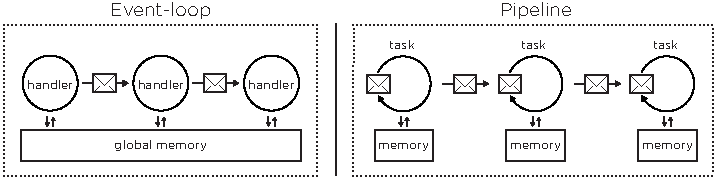
\includegraphics[page=1]{../resources/models-difference.pdf}}{
    \includegraphics[page=2]{../resources/models-difference.pdf}}{
  }
\end{figure}

% \begin{figure}
%   \centering
%   \textfig{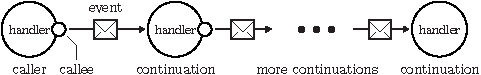
\includegraphics[width=0.8\linewidth]{../resources/cont-chain.pdf}}
% \end{figure}

\paragraph{Fluxional execution model}

The fluxional execution model is targeted by a more efficient programming language.
It executes an application expressed as a network of independent application parts called fluxions.
The fluxions communicate by messages, and form a pipeline similarly to the handlers of the event-driven execution model.
They are executed in parallel to distribute the computation across several cores and increase the performance efficiency.
They rely on isolated memory store, called context to allow this parallel execution.
When several fluxions need to rely on the same memory store, they are grouped, and executed sequentially.
When they are independent, they are isolated to increase performance efficiency.

The similarity between the event-driven execution model and the fluxional execution model leads to the equivalence presented in the next paragraph.
With this equivalence, the versatility of fluxions allows to progressively adapt the implementation from a productive, single event-loop, toward an efficient pipeline.

\subsection{Equivalence}

The equivalence describes the transformation from an application targeting the event-driven execution model to execute them in parallel in the fluxional execution model.
This transformation involves two steps: the extraction and isolation of the stages to form the pipeline.

\paragraph{Stage Extraction} \label{chapter7:summary:extraction}

The first step is the identification and extraction of the stages.
The equivalence identifies rupture points between stages.
A rupture point is an asynchronous call without subsequent synchronization with the caller.
It indicates a rupture in the synchronous control-flow, and the boundaries between two handlers.
The upstream handler is the one calling the asynchronous call, the downstream handler is the callback provided to the asynchronous call.

There are two kinds of rupture points: \textit{start} and \textit{post}.
\textit{Start} rupture points directly receives the input stream, and start the execution of the chain of stages for each new datum in the stream.
\textit{Post} rupture points indicates a continuity in the chain of stages.

The difficulty in this compilation step is to identify the asynchronous functions indicating the stages.
Because of the dynamic behaviors of Javascript, it is impossible to statically detect these functions.
The compiler implemented from the equivalence is currently unable to reliably detect them.
Instead the compiler rely on the developer to provide a list of asynchronous function names to extract.

\paragraph{Stage Isolation} \label{chapter7:summary:isolation}

% After the extraction of this pipeline,
The second step is the identification of the memory interdependencies between stages.
It intends to isolate the stages so they can be executed in parallel.
The common memory is replaced by message-passing, following some rules to preserve consistency.
\begin{itemize}
\item If a stage needs to hold a variable from one request to the other, this variable is stored in its context.
\item If a downstream stage needs to read a variable from an upstream stage, the variable is sent as part of the message communication.
\item If two stages needs to share a variable, they are grouped on the same execution node to safely share parts of their context.
Their executions are not parallelized to avoid conflicting accesses.
\end{itemize}

The difficulty in this step is to identify the memory dependencies between stages.
The dynamic behaviors of Javascript makes it impossible to statically identify aliasing in the memory.
The compiler implemented from the equivalence is currently unable identify these interdependencies.
It relies on manual manipulations to complete the transformation.

\separator

These difficulties are details in further details in the next section.
It then presents some perspectives to overcome these limitations.